% Beamer do material do curso de Verão (2015) do IME-USP
% Introdução ao Projeto de Jogos
%
% Baseado no template LaTeX das apresentações do LIDET versão 2
% (https://github.com/luigivieira/LIDET)
%

\providecommand\classopts{}
\expandafter\documentclass\expandafter[table, usenames, svgnames, dvipsnames, \classopts]{beamer}

\usepackage{etex}
\usepackage{beamerthemeshadow}
\usepackage[portuguese]{babel}
\usepackage[utf8]{inputenc}
\usepackage[absolute,overlay]{textpos}
\usepackage{array}
\usepackage{framed}
\usepackage{booktabs}
\usepackage[compatibility=false]{caption}
\usepackage{subcaption}
\usepackage{outlines}
\usepackage{ulem}
\usepackage{xcolor,colortbl}
\usepackage{ragged2e}
\usepackage{tikz}
\usepackage{multirow}

% ---------------------------------------------------------------------------- %
% Presentation definitions
% ---------------------------------------------------------------------------- %
\usetheme{Luebeck}
\hypersetup{pdfpagemode=FullScreen} % Starts the presentation in full screen

% layout
\setbeamerfont{frametitle}{size=\normalsize}
\setbeamerfont{title}{size=\normalsize}
\beamertemplatenavigationsymbolsempty
\setbeamertemplate{bibliography item}[text]%
\setbeamertemplate{headline}{} % Remove upper bar

% colors
\definecolor{lidet_orange}{rgb}{0.9, 0.49, 0.09}
\definecolor{lidet_black}{rgb}{0.2, 0.2, 0.2}

\setbeamercolor{title}{bg=lidet_orange}
\setbeamercolor{structure}{bg=white, fg=lidet_orange}
\setbeamercolor{normal text}{fg=black}
\setbeamercolor{section in head/foot}{fg=white, bg=lidet_black}
\setbeamercolor{postit}{fg=white, bg=lidet_orange!90!lidet_black}

% shadow
\makeatletter
\pgfdeclareverticalshading[black,bg]{bmb@shadow}{200cm}{%
  color(0bp)=(lidet_black!25); color(4bp)=(black!50!bg); color(8bp)=(black!50!bg)}
\pgfdeclareradialshading[black,bg]{bmb@shadowball}{\pgfpointorigin}{%
  color(0bp)=(black!50!bg); color(4bp)=(lidet_black!25)}
\pgfdeclareradialshading[black,bg]{bmb@shadowballlarge}{\pgfpointorigin}{%
  color(0bp)=(black!50!bg); color(4bp)=(black!50!bg); color(8bp)=(lidet_black!25)}
%
\makeatother

% Captions for images and tables
\setlength{\abovecaptionskip}{5pt plus 5pt minus 5pt}
\setlength{\belowcaptionskip}{5pt plus 5pt minus 5pt}
\captionsetup[figure]{font=scriptsize,labelfont=scriptsize}
\captionsetup[table]{font=scriptsize,labelfont=scriptsize}
\captionsetup{labelformat=empty,labelsep=none}

% Dimensions for table rules
\setlength\heavyrulewidth{0.1em} 
\setlength\lightrulewidth{0.01em}
\setlength\belowrulesep{0.10ex}
\setlength\aboverulesep{0.10ex}

% Define macros to mark the begining and ending of references
% Basically, handles the automatically spanned frames (due to parameter allowframebreaks)
% as backup frames, so they do not influence in the frame numbering
\newcommand{\referencesbegin}{
   \newcounter{framenumberappendix}
   \setcounter{framenumberappendix}{\value{framenumber}}
}
\newcommand{\referencesend}{
   \addtocounter{framenumberappendix}{-\value{framenumber}}
   \addtocounter{framenumber}{\value{framenumberappendix}} 
}

% Adjust footnotes to not overlap the footbar
\addtobeamertemplate{footnote}{}{\vspace{1.0ex}}
\let\oldfootnotesize\footnotesize
\renewcommand*{\footnotesize}{\oldfootnotesize\tiny}

% Redefine the quote environment so short quotes are not broken easily
\renewenvironment{quote}
	{\list{}{\leftmargin1em\rightmargin\leftmargin}%
	\item\relax}
	{\endlist}

% Section frames (that appear before each section)
\AtBeginSection[] 
{
	{
		\setbeamertemplate{footline}{} % Hide the footline locally for these frames
		\begin{frame}<beamer>[noframenumbering]
			\begin{center}
				\begin{tikzpicture}
					\node[align=left, left color=lidet_orange, right color=lidet_orange, draw, rounded corners, minimum width=10cm, minimum height=1cm] {\color{white} \textbf{\insertsectionhead}};
				\end{tikzpicture}
			\end{center}
			\footnotesize{ \tableofcontents[currentsection, hideothersubsections] }
		\end{frame}
	}
}

\AtBeginSubsection[]
{
    \begin{frame}
        \centering
        \Large
        \textbf{\insertsubsection}
    \end{frame}
}

\AtBeginSubsubsection[]
{
    \begin{frame}
        \centering
        \large
        \insertsubsection
        \vskip 1em
        \Large
        \textbf{\insertsubsubsection}
    \end{frame}
}

\DeclareGraphicsExtensions{.pdf,.jpg,.png}
\graphicspath{{./images/}}

% ---------------------------------------------------------------------------- %
% Presentation title, author and institution
% ---------------------------------------------------------------------------- %
\newcommand{\lessontitle}{Aula 5 - Executando testes e avaliações}
\title{\textbf{Introdução ao Projeto de Jogos}}
\subtitle{{\small \lessontitle}}

\newcommand{\autores}{Luiz C. Vieira, Vinícius K. Daros}
\author[\autores]{\scriptsize
    Luiz Carlos Vieira e Vinícius Kiwi Daros\\
    \{luigivieira,vinicius.k.daros\}@gmail.com
}

\newcommand{\lidet}{LIDET (IME - USP)}
\institute[\lidet]{\\[1.0mm]
Curso de Verão (2015)\\
Departamento de Ciência da Computação}

\date{{\tiny 16 de Janeiro de 2015}}

% ---------------------------------------------------------------------------- %
% Presentation content
% ---------------------------------------------------------------------------- %

% ---------------------------------------------------------------------------- %
\begin{document}
% ---------------------------------------------------------------------------- %

% ---------------------------------------------------------------------------- %
% First Slide (index 0) = cover
% ---------------------------------------------------------------------------- %

{%\usebackgroundtemplate{}} 
\begin{frame}[plain, noframenumbering]

	\begin{columns}[c]
		\column{0.2\textwidth}
			\hspace*{-1.5em}
			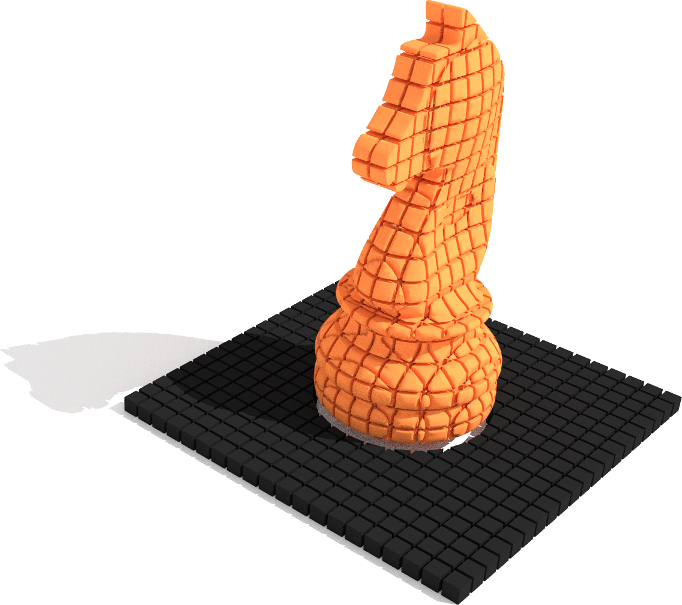
\includegraphics[width=0.35\paperwidth]{side_bar}\\
		\column{0.01\textwidth}
		\column{0.70\textwidth}
			\titlepage
			\hspace*{+0.5em}
			\begin{center}
				
\includegraphics[height=1.0cm]{lidet-logo}\\
				
\includegraphics[height=1.0cm]{ime-logo}\\
			\end{center}
	\end{columns}
	%\addtocounter{framenumber}{-1}
\end{frame}
}

% ---------------------------------------------------------------------------- %
% Other Slides (index from 1 onwards)
% ---------------------------------------------------------------------------- %

% setup navigation symbols and footline
\setbeamertemplate{navigation symbols}{}
\makeatletter
\setbeamertemplate{footline}{%
    \leavevmode%
    \hbox{%
        \begin{beamercolorbox}[wd=0.28\paperwidth,ht=4ex,dp=1ex,left,%
                               leftskip=2ex]{author in head/foot}%
            \usebeamerfont{title in head/foot}
            \insertdate\newline%
            \vskip 0.6ex%
            \autores
        \end{beamercolorbox}%
        \begin{beamercolorbox}[wd=0.53\paperwidth,ht=4ex,dp=1ex,center]%
                              {author in head/foot}%
            \usebeamerfont{author in head/foot}\lessontitle%
        \end{beamercolorbox}%
        \begin{beamercolorbox}[wd=0.19\paperwidth,ht=4ex,dp=1ex,right,%
                               rightskip=2ex]{author in head/foot}%
            \insertframenumber{}/\inserttotalframenumber \newline
            \lidet%
        \end{beamercolorbox}%
    }%
    \vskip 4cm%
}
\makeatother

% ---------------------------------------------------------------------------- %
\begin{frame}[plain]
\frametitle{\textbf{Agenda}}

	\hspace*{+4.0em}
	\footnotesize{ \tableofcontents }
\end{frame}

% ---------------------------------------------------------------------------- %
\section{Planejamento}
% ---------------------------------------------------------------------------- %

% ------------------------------
\begin{frame}{\textbf{O plano pra hoje}}

	As atividades de hoje são as seguintes:

	\begin{outline}[enumerate]
		\1 Aula expositiva
			
		\vspace{1em}

		\1 Sessão de \textit{playtesting}

		\vspace{1em}

		\1 Intervalo

		\vspace{1em}

		\1 Sessão de refatoração

		\vspace{1em}

		\1 Sessão de \textit{playtesting}

		\vspace{1em}

		\1 Sessão de \textit{pitches}

	\end{outline}

\end{frame}

% ---------------------------------------------------------------------------- %
\section{Heurísticas de projeto}
% ---------------------------------------------------------------------------- %

% ------------------------------
\begin{frame}{\textbf{Heurísticas}}

	\begin{outline}

		\1 \textit{Heurística} é uma palavra de origem grega, que significa ``encontrar'' ou ``descobrir''\footnote{Fonte: \url{http://pt.wikipedia.org/wiki/Heur\%C3\%ADstica}}
			\2[-] {\scriptsize mesma origem de \textit{Eureca} (``encontrei'')}

		\vspace{1em}

		\1 Método ou processo criado com o objetivo de encontrar uma solução para um problema
			\2[-] {\scriptsize envove substituir questões difíceis por outras mais fáceis}
			\2[-] {\scriptsize de forma a encontrar soluções viáveis, ainda que imperfeitas}

		\vspace{1em}

		\1 Exemplo clássico: chave do carro perdida
			\2[-] {\scriptsize ao invés de procurar em todos os locais possíveis (problema difícil)...}
			\2[-] {\scriptsize ...a busca é realizada nos locais \emph{mais prováveis} (problema mais fácil)}

	\end{outline}

\end{frame}

% ------------------------------
\begin{frame}{\textbf{O uso de heurísticas}}

	As heurísticas servem para dois propósitos:

	\begin{outline}

		\1 Servir como melhoras práticas para as escolhas de projeto

		\vspace{1em}

		\1 Servir como pontos de questionamento para a avaliação com protótipos

	\end{outline}

\end{frame}

% ------------------------------
\begin{frame}{\textbf{Exemplo de heurísticas: Lentes de Game Design}}

	\begin{figure}
		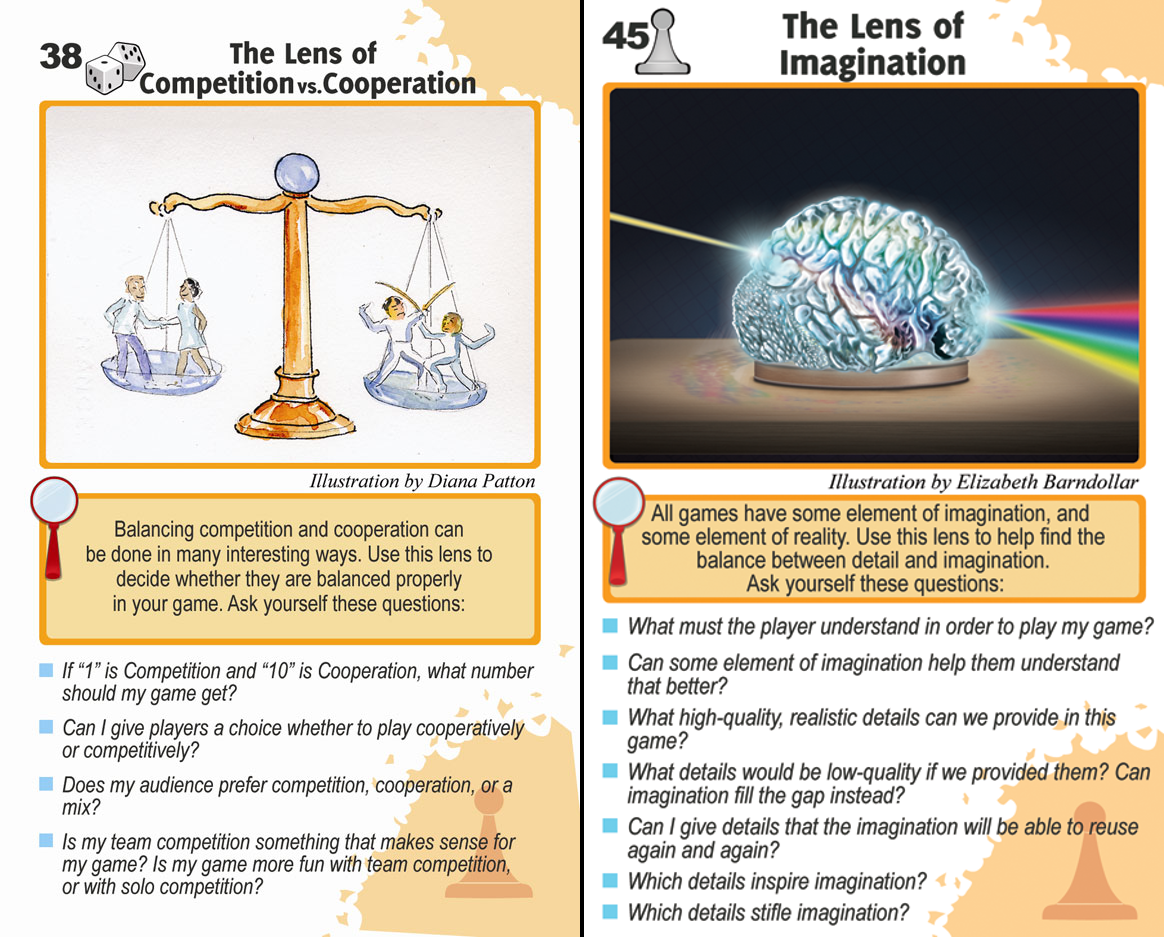
\includegraphics[height=4.5cm]{game-design-lenses}
		\caption{\tiny\textbf{Exemplos das lentes de game design} \copyright{2008} Jesse Schell\footnote{\url{http://www.amazon.com/The-Art-Game-Design-Lenses/dp/0615218288}}}
	\end{figure}

	\begin{block}{Lembrete}
		\centering
		O aplicativo gratuito (Android) pode ser baixado de:\\
		{\scriptsize \url{https://play.google.com/store/apps/details?id=com.schellgames.deckoflenses&hl=pt_BR}}
	\end{block}

	\vspace{1em}

\end{frame}

% ------------------------------
\begin{frame}{\textbf{Exemplo de heurísticas: GameFlow}}

	\begin{table}
		\scriptsize
		\setlength{\tabcolsep}{1pt}
		\renewcommand{\arraystretch}{1.5}
		\caption{\textbf{Algumas das heurísticas do modelo GameFlow} \cite{Sweetser2005}}

		\begin{tabular}{p{0.2\textwidth}p{0.8\textwidth}}

			\toprule
			\textbf{Elemento} & \textbf{Critério}\\
			\midrule
			\multirow{3}{*}{Desafio}  & -- os desafios devem ser equiparados às habilidades do jogador\\
									  & -- o jogo deve prover diferentes níveis de dificuldade para diferentes jogadores\\
									  & -- o nível do desafio deve aumentar progressivamente\\[1em]
			\midrule

			\multirow{4}{*}{Controle} & \\ & -- os jogadores devem ter a sensação de controle sobre seus personagens ou unidades, movimento, e interações no jogo\\
									  & -- os jogadores devem ter a sensação de controle sobre a interface e os dispositivos de entrada\\
									  & -- os jogadores não devem ser capazes de cometer erros que são prejudiciais ao jogo\\
			\bottomrule
		
		\end{tabular}

	\end{table}

\end{frame}

% ---------------------------------------------------------------------------- %
\section{Playtesting}
% ---------------------------------------------------------------------------- %

% ------------------------------
\begin{frame}{\textbf{Por que testar?}}

	Os testes podem ter diferentes propósitos:

	\begin{outline}
		\1 Avaliar o potencial de diversão das ideias de design existentes (\textit{gameplay})
			\2[-] {\scriptsize e coletar novas ideias!}
			
		\vspace{1em}
			
		\1 Avaliar a implementação do jogo sob aspectos ``utilitários'' (jogabilidade) e estéticos (``juiciness'')
			\2[-] {\scriptsize símbolos e indicações utilizadas}
			\2[-] {\scriptsize percepção dos objetivos e do feedback das ações}
			\2[-] {\scriptsize ergonomia dos dispositivos de interface}
			\2[-] {\scriptsize balanceamento de dificuldade -- individual e entre jogadores}
			\2[-] {\scriptsize empatia com personagens, preferências por cores, etc}
		
		\vspace{1em}

		\1 Avaliar a implementação do jogo sob o ponto de vista técnico
			\2[-] {\scriptsize durabilidade de componentes}
			\2[-] {\scriptsize erros de codificação (para jogos digitais)}
			\2[-] {\scriptsize condições de uso não previstas}
		
	\end{outline}

\end{frame}

% ------------------------------
\begin{frame}{\textbf{Prototipação em Papel}}

	\begin{figure}
	    \centering
        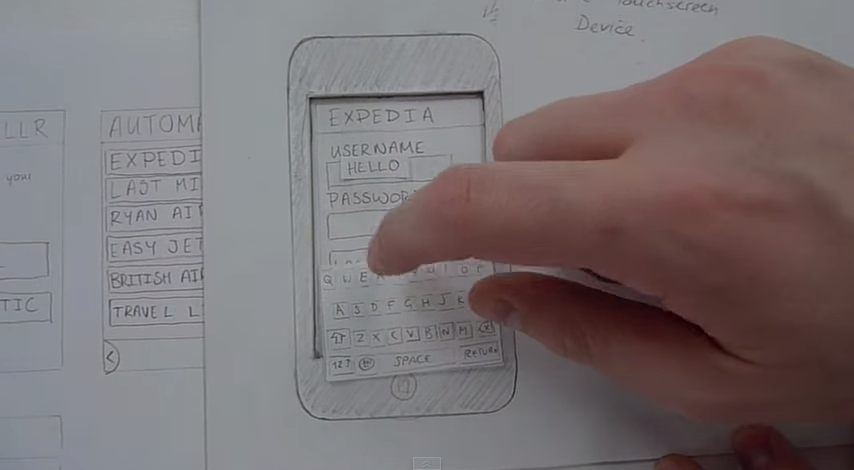
\includegraphics[width=0.8\paperwidth]{paper-prototype}
        \caption{\textbf{Exemplo de protótipo em papel}, Travellr App\footnote{\url{https://www.youtube.com/watch?v=_5FGeSQ7DBU}}}
    \end{figure}

    \begin{center}
    	Video 13
    \end{center}

    \vspace{2em}

\end{frame}

% ------------------------------
\begin{frame}{\textbf{O Mágico de Oz}}

	\begin{figure}
	    \centering
        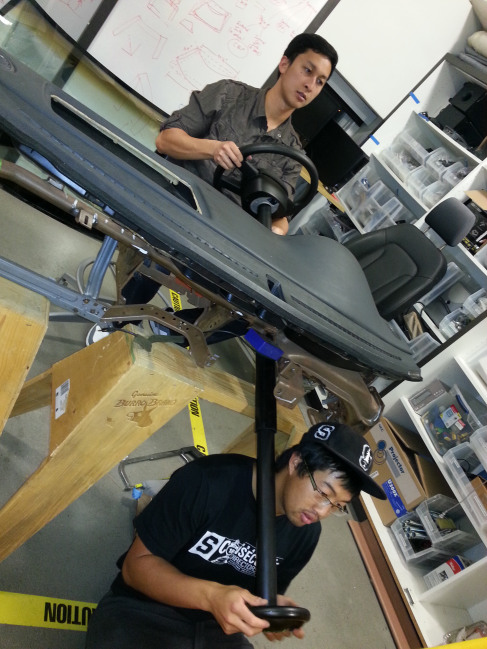
\includegraphics[height=0.7\paperheight]{wizard-of-oz}
        \caption{\textbf{Avaliação do mecanismo de transição de um carro automatizado}, Stanford Jr Team\footnote{\url{http://310valeo.wordpress.com/2013/11/20/cfp-prototyping/}}}
    \end{figure}

\end{frame}

% ------------------------------
\begin{frame}{\textbf{Observação, questionários e entrevistas}}

	\begin{outline}
		\1 Observação (de jogadores jogando), questionários e entrevistas são ferramentas muito úteis
			\2[-] {\scriptsize mas alguns cuidados são necessários}

		\vspace{1em}

		\1 A observação pode ter efeitos sobre a experiência
			\2[-] {\scriptsize os jogadores podem se sentir incomodados, desejar impressionar ou não desejar magoar o observador}
			
		\vspace{1em}
			
		\1 Questionários interrompem a experiência ou podem não capturar o ``calor do momento''
			\2[-] {\scriptsize além disso, deve-se procurar não induzir respostas}
		
		\vspace{1em}

		\1 Entrevistas também interrompem a experiência
			\2[-] {\scriptsize e diminuem o anonimato}
	\end{outline}

\end{frame}

% ------------------------------
\begin{frame}{\textbf{GEQ: Game Experience Questionnaire}}

	\begin{outline}
		\1 Dois questionários padronizados produzido pela Universidade de Tecnologia de Eindhoven (Holanda)
			\2[-] {\scriptsize baseado em todos os assuntos estudados até esta aula}
			\2[-] {\scriptsize para ser utilizado durante e após as sessões de jogos}

		\vspace{1em}

		\1 Contém questões \emph{Likert} para avaliar oito aspectos da experiência
			\2[-] {\scriptsize imersão}
			\2[-] {\scriptsize fluxo}
			\2[-] {\scriptsize competência}
			\2[-] {\scriptsize emoções positivas e negativas}
			\2[-] {\scriptsize tensão}
			\2[-] {\scriptsize desafio}
			\2[-] {\scriptsize presença social}
	\end{outline}

\end{frame}

% ------------------------------
\begin{frame}{\textbf{GEQ: Game Experience Questionnaire}}

	Exemplos de questões:

	\vspace{1em}

	\begin{outline}
		\0 \textit{Por favor indique como se sentiu enquanto jogou o jogo para cada item, na seguinte escala}:\\
		\0 \textit{de forma alguma (0), levemente (1), moderadamente (2), bastante (3), extremamente (4)}

		\vspace{1em}

		\1 Eu me senti contente
		\1 Eu achei que foi divertido
		\1 Eu pensei sobre outras coisas
		\1 Eu me senti capaz/competente
		\1 Foi esteticamente agradável
		\1 Eu esqueci de tudo ao meu redor
		\1 Eu fui bem no jogo
		\1 Eu tive que colocar muito esforço no jogo
	\end{outline}

\end{frame}

% ------------------------------------------
% References
% ------------------------------------------

\referencesbegin
\begin{frame}[plain, allowframebreaks]
	\frametitle{\textbf{References}}
	\bibliographystyle{abbrv}
	{\tiny \bibliography{bibliography}}
\end{frame}
\referencesend

\end{document}